\subsection{Acquisition of Agricultural Remote Sensing Data}

\subsubsection{Data Acquisition Platforms}
The acquisition of agricultural remote sensing data primarily relies on three platforms: satellite remote sensing, UAV\cite{Unmanned27:online} remote sensing, and ground sensors\cite{mandalImpactAgriculturalManagement2022}. Each of these platforms has its own advantages and disadvantages, catering to different application needs.

\begin{figure}[htbp!]
    \centering
    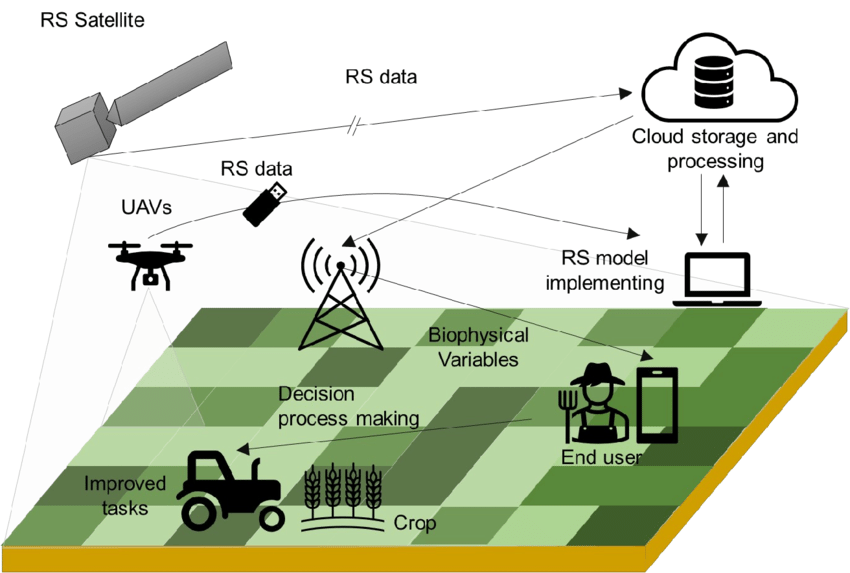
\includegraphics[width=0.35\textwidth]{figs/remote_sensing.png}
    \caption{Remote Sensing and Agricultural}
\end{figure}

\paragraph{Satellite Remote Sensing}

Satellite remote sensing is the most commonly used method for acquiring agricultural remote sensing data. Remote sensors mounted on satellites orbiting the Earth can regularly and continuously obtain large-scale surface information.

Satellite remote sensing has many advantages. Satellite remote sensing can cover global areas, suitable for monitoring large-scale farmland. Most remote sensing satellites can regularly obtain data, suitable for long-term monitoring of crop growth dynamics. Many satellites are equipped with multispectral sensors that can obtain data in various bands such as visible light, near-infrared, and shortwave infrared, suitable for various agricultural applications\cite{sahooHyperspectralRemoteSensing2015}.


Here are some application cases about this kind of sensors.

Landsat Series\cite{Landsatp77:online}: Jointly launched by the U.S. Geological Survey (USGS) and NASA, the Landsat series satellites provide medium-resolution multispectral data widely used in land use and crop monitoring.

Sentinel Series\cite{Sentinel88:online}: The European Space Agency (ESA)'s Sentinel series satellites include both multispectral and radar remote sensing data, suitable for agriculture, environmental monitoring, and other applications.

MODIS\cite{MODISWeb11:online}: The MODIS sensors on NASA's Terra and Aqua satellites provide high temporal resolution, medium-to-low resolution data suitable for large-scale agricultural monitoring.

%『插入图像:对应的卫星图像』

\paragraph{UAV Remote Sensing}

UAV (unmanned aerial vehicle)\cite{Unmanned27:online}(Fig.\ref{fig:UAVs}) remote sensing is a highly flexible data acquisition method. UAVs equipped with high-resolution sensors can fly at low altitudes to obtain high-precision surface information.

As they fly at low altitudes, UAVs\cite{Unmanned27:online} can capture high-resolution images suitable for detailed farmland monitoring. Moreover, UAV\cite{Unmanned27:online} flight plans can be flexibly adjusted according to needs, adapting to different task requirements. Compared to satellite remote sensing, UAV\cite{Unmanned27:online} remote sensing is less costly, suitable for small-scale agricultural applications.

Here are some application cases about this kind of sensors.

Crop Health Monitoring\cite{javedPerformanceRelationshipFour2021}: By acquiring high-resolution multispectral and thermal infrared images, UAVs\cite{Unmanned27:online} can monitor the growth and health of crops, identifying pests and nutrient deficiencies early.

Precise Farmland Management: UAV\cite{Unmanned27:online} remote sensing data can be used for precise farmland management, such as targeted fertilization and irrigation, optimizing the use of agricultural resources.

\begin{figure*}[htbp!]
    \centering
    \begin{subfigure}[b]{0.3\textwidth}
        \centering
        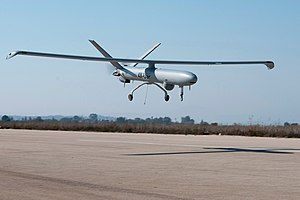
\includegraphics[height=0.15\textheight]{figs/U1.jpg}
        \caption{Elbit Systems Hermes-450}
    \end{subfigure}
    \begin{subfigure}[b]{0.3\textwidth}
        \centering
        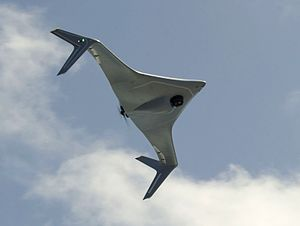
\includegraphics[height=0.15\textheight]{figs/U2.jpg}
        \caption{Northrop Grumman Bat}
    \end{subfigure}
    \begin{subfigure}[b]{0.3\textwidth}
        \centering
        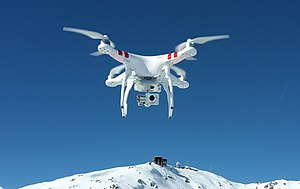
\includegraphics[height=0.15\textheight]{figs/U3.jpg}
        \caption{DJI Phantom quadcopter UAV}
    \end{subfigure}
    \caption{UAVs (Unmanned Aerial Vehicles)}
    \label{fig:UAVs}
\end{figure*}

\paragraph{Ground Sensors}

Ground sensors are devices installed on the ground to monitor various environmental parameters of farmland in real-time. Common ground sensors include soil moisture sensors, weather stations, and chlorophyll sensors.

Different from satellite remote sensing, ground sensors can collect data in real-time, which are suitable for dynamic monitoring\cite{khanalRemoteSensingAgriculture2020}. Ground sensors can also obtain high-precision environmental parameters such as soil moisture and temperature. Many ground sensors directly contact the target object, providing highly reliable data.

Here are some application cases about this kind of sensors.

Soil Moisture Monitoring: Soil moisture sensors can monitor the water content of farmland soil in real-time, providing data support for precision irrigation.

Meteorological Monitoring: Weather stations can monitor meteorological parameters such as temperature, precipitation, and wind speed, providing weather forecasts and risk assessments for agricultural production.

\subsubsection{Spatiotemporal Resolution Requirements for Data Acquisition}

The spatiotemporal resolution requirements of agricultural remote sensing data depend on specific application needs. Spatiotemporal resolution refers to the spatial and temporal resolution of remote sensing data.

\paragraph{Spatial Resolution}

Spatial resolution refers to the smallest size of the surface object that the sensor can distinguish. High spatial resolution data can provide more detailed surface information, suitable for precise farmland management; low spatial resolution data are suitable for large-scale regional monitoring.
Crop classification requires medium to high spatial resolution (10-30 meters) data to accurately identify different types of crops. Pest monitoring requires high spatial resolution (<10 meters) data to detect and locate pest-infested areas early. Soil moisture monitoring generally requires medium to low spatial resolution (>30 meters) data, which can usually meet the needs.

\paragraph{Temporal Resolution}

Temporal resolution refers to the frequency at which the sensor acquires data. High temporal resolution data can provide continuous time series information, suitable for dynamic monitoring; low temporal resolution data are suitable for monitoring changes over long time scales.
Crop growth monitoring requires high temporal resolution (daily or weekly) data to detect and address issues arising during the growth process promptly.
Agricultural disaster (e.g., drought, flood) monitoring requires high temporal resolution data to quickly assess the impact of the disaster and develop response measures.
Long-term change monitoring of land use and climate change impacts on agricultural production can use low temporal resolution (monthly or yearly) data.

In conclusion, the acquisition of agricultural remote sensing data relies on satellite remote sensing, UAV remote sensing, and ground sensors, each with its unique advantages and applicable scope. Choosing appropriate spatiotemporal resolutions according to specific application needs can effectively enhance the application effectiveness of remote sensing data. By comprehensively utilizing data from different platforms and resolutions, it is possible to achieve comprehensive, detailed, and dynamic monitoring and management of farmland, providing strong technical support for precision agriculture and sustainable agricultural development.